\documentclass[10pt,twocolumn]{article}
\usepackage{graphicx}
\usepackage{amsmath,amssymb,times,cite}
\usepackage{hyperref}
\usepackage{listings}
\usepackage{color}
\definecolor{mygreen}{rgb}{0,0.6,0}
\definecolor{mygray}{rgb}{0.5,0.5,0.5}
\definecolor{mymauve}{rgb}{0.58,0,0.82}
\lstset{ 
  backgroundcolor=\color{lightblue},   % choose the background color; you must add \usepackage{color} or \usepackage{xcolor}; should come as last argument
  basicstyle=\footnotesize,        % the size of the fonts that are used for the code
  breakatwhitespace=false,         % sets if automatic breaks should only happen at whitespace
  breaklines=true,                 % sets automatic line breaking
  captionpos=b,                    % sets the caption-position to bottom
  commentstyle=\color{mygreen},    % comment style
  deletekeywords={...},            % if you want to delete keywords from the given language
  escapeinside={\%*}{*)},          % if you want to add LaTeX within your code
  extendedchars=true,              % lets you use non-ASCII characters; for 8-bits encodings only, does not work with UTF-8
  frame=false,	                   % adds a frame around the code
  keepspaces=true,                 % keeps spaces in text, useful for keeping indentation of code (possibly needs columns=flexible)
  keywordstyle=\color{blue},       % keyword style
  language=Python,                 % the language of the code
  morekeywords={*,...},            % if you want to add more keywords to the set
 % numbers=left,                    % where to put the line-numbers; possible values are (none, left, right)
  numbersep=5pt,                   % how far the line-numbers are from the code
 % numberstyle=\tiny\color{mygray}, % the style that is used for the line-numbers
  rulecolor=\color{lightblue},         % if not set, the frame-color may be changed on line-breaks within not-black text (e.g. comments (green here))
  showspaces=false,                % show spaces everywhere adding particular underscores; it overrides 'showstringspaces'
  showstringspaces=false,          % underline spaces within strings only
  showtabs=false,                  % show tabs within strings adding particular underscores
  stepnumber=2,                    % the step between two line-numbers. If it's 1, each line will be numbered
  stringstyle=\color{mymauve},     % string literal style
  tabsize=2,	                   % sets default tabsize to 2 spaces
  %title=\lstname                   % show the filename of files included with \lstinputlisting; also try caption instead of title
}
%Our symbols
\DeclareMathOperator{\diag}{diag}

%Bold symbols
\newcommand{\bg}[1]{\boldsymbol{#1}} %Bold Greek letters
\newcommand{\bm}[1]{\mathbf{#1}} %Bold vectors and matrices

%Transpose symbol
\newcommand\T{{\mathpalette\raiseT\intercal}}
\newcommand\raiseT[2]{%
\setbox0\hbox{$#1{#2}$}\raise\dp0\box0}

%================================================================
\usepackage{algorithm,algorithmic}
% Algorithmic modifications
\makeatletter
\newcommand{\ALOOP}[1]{\ALC@it\algorithmicloop\ #1%
  \begin{ALC@loop}}
\newcommand{\ENDALOOP}{\end{ALC@loop}\ALC@it\algorithmicendloop}
\renewcommand{\algorithmicrequire}{\textbf{Input:}}
\renewcommand{\algorithmicensure}{\textbf{Output:}}
\newcommand{\algorithmicbreak}{\textbf{break}}
\newcommand{\BREAK}{\STATE \algorithmicbreak}
\makeatother
%================================================================

\usepackage{booktabs}
\usepackage[table]{xcolor}
\newcommand{\head}[1]{\textnormal{\textbf{#1}}}
\newcommand{\normal}[1]{\multicolumn{1}{l}{#1}}
\definecolor{lightgray}{gray}{0.9}
\definecolor{lightblue}{rgb}{0.93,0.95,1.0}

\title{\Large\textbf{Factors Affecting Marriage Dissolution in the U.S.}}
\author{Raed Abdel Sater - Student ID: 40075908\\
 Risk Analysis for Information and Systems Engineering - INSE 6320\\
Concordia Institute for Information Systems Engineering
}
\date{}
\renewcommand{\topfraction}{0.85}
\renewcommand{\textfraction}{0.1}
\renewcommand{\floatpagefraction}{0.75}

\topmargin      -20.0mm
\oddsidemargin  -11.0mm
\evensidemargin -11.0mm
\textheight     242.0mm
\textwidth      183.0mm
\columnsep        4.1mm
\parindent        1.0em
\headsep          6.3mm
\headheight        12pt
\lineskip           1pt
\normallineskip     1pt

%Bold symbols
%\usepackage{bm} %Load bm package
%\newcommand{\bv}[1]{\boldsymbol{\mathbf{#1}}} %Bold vectors/matrices
\begin{document}
\maketitle
\begin{abstract}
This project investigates the factors affecting the marriage dissolution in the U.S. and analyzes covariates by the geographical region, education level, income, children, couple ethnicity and poverty percentage in each state. Provincial data from Princeton University  database\cite{Princeton2017University} has been used along with a part of the United States Census Bureau dataset on poverty, one of the largest ever databases covering all demographic information in the states\cite{Census2018Bureau}. Using marital information of 3371 couples distributed in 4 different states to investigate marriage patterns among the richest states of New Hampshire and Maryland and compare it to the situation of couples in the poorest states in Alabama and Mississippi according to the poverty percentage. We describe and predict marriage survival time based on an interval of time between the years 1970 and 2016. A lot of observations have been made during the analysis of data, the influence of several covariates, especially education level and income have been given a special attention to understand their effects on marriage. In addition to these results, the paper presents an introduction to survival analysis methods, hazard function, cumulative hazard and regression models and their corresponding implementation in Python using Lifelines package. 

Women ages at marriage has been omitted in our study due to the lack of information on women participating in this survey, only husband ethnicity and education was taken into consideration which create one of the limitations. The study showed that Educated husbands have higher chances of marriage dissolution than the illiterate ones. Results suggest that dissolution rates are quite higher in Alabama, Mississippi and few regions of Maryland.
\end{abstract}

\bigskip
\noindent\textbf{Keywords}:\,Survival analysis; Hazard rate; Cox Proportional Model;Marriage Patterns; Kaplan-Meier; Aalan additive model; Linear regression; Correlation; Concordance index...
\section{Introduction}
To understand the marriage as an essential social event which changes a person status or identity after a marital union, a lot of factors affecting this phenomenon needed to be studied in depth. Marriage can provide mental security by giving people a greater sense of care and emotional support by their partners allowing them to fulfill several challenges and play multiple social roles\cite{berkman2000social}. It's proved scientifically that married people have higher levels of psychological and physical well-being than individuals who are single, separated or divorced\cite{overbeek2006longitudinal}. During the past few decades it has been seen that industrial development has powerful influence on family dynamics in many parts of the U.S. Several changes are occurring in the family patterns,observations ranged from changes in marriage to fertility practices,delayed marriages, divorce and remarriage, changing living
arrangements, changes of individual partner's choice, and better involvement for the women's role in the society. However, the increased rate of divorce and changes in marriage pattern remains one of the marked demographic trends observed in twentieth century\cite{grundy2005reciprocity}. Divorce recently draws the attention of social and data scientists as it is a social phenomenon deeply rooted in the socio economic status and cultural factors of society that varies across the culture and over the time. In most of the western countries and the U.S. divorce rates have shown an increasing trend\cite{cherlin2010demographic}. Most of the European countries are experiencing two to five times higher divorce rates, than the in the 1960. There is a universal trend of increasing divorce rates has been seen in Europe since 1970s \cite{billari2010towards}. Scientists stated that the way industrialization and urbanization have brought changes in marriage pattern in the states under the form of different patterns depending on each state and each couple.
Industrialization affecting income level and
education lead to a change in society; family composition and participation of women into labor force which led in the majority of cases to unhappy marriages \cite{laland2006niche}. Contrary to the general belief the authors in \cite{hirschman2003cultural} opined that it is not always true that by rising urbanization there is rise in marriage dissolution rates. Studies proved that traditionally high divorce countries such as  Malaysia, have experienced a decline in divorce with modernization and development. The frequency and pattern of divorce varies within and across the countries. In his study \cite{hammer2006scenes}, the World Bank made a comparison between Australian and American couple’s divorce and concluded that Australians have less frequent divorces than Americans, and generally after a much longer duration of marriage. In parallel, divorce and separation in the U.S. occur more frequently among black and poor couples \cite{kennedy2014breaking}. In its early report, UNICEF \cite{unicef2005early} found that developing countries have a higher divorce rate in rural areas, than in urban areas in all the age groups where parents encourage the marriage of their daughters while they are still children. In the states,on contrary to that, divorce is higher in case of urban women than in the rural areas \cite{rennison2000intimate}. Probabilities of divorce are high during the earlier years of marriage and declines sharply with the increase of marital duration \cite{vanlaningham2001marital}. There are various consequences of rising divorce rates on individual level as well as at the family level. The project tries to stratify all possible factors in order to get full understanding of the studied event
\section{Divorce in Context of the U.S.}
In the U.S., marriage has always been seen as a dynamic social event. In the past several decades marriage system has experienced various changes as a result of prosperity,socioeconomic development, improvement in education, dramatic increase in age at marriage of both the sexes, changes on attitude towards marriage, love-marriages,same-sex marriages, divorce and separation has been observed \cite{alba1986patterns}. The growing role of women and their role in the modern society has opened new avenues and challenges. In consequence, unhappy marriages are being terminated by divorce, which is an effective alternative initiated by legislative action and strengthened by legal sanction. The divorce rate varies from couple to couple and it is affected by several social and economic factors, Figure 1 shows the distribution of divorce among 3371 couples in the  4 following states: New Hampshire, Maryland, Mississippi and Alabama where the data were collected.
\begin{figure}[!htb]
\centering
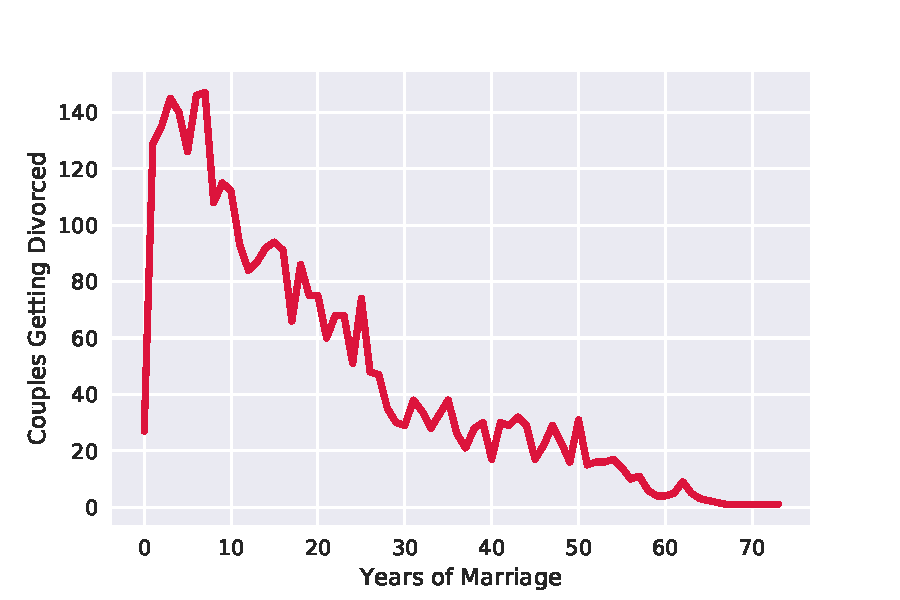
\includegraphics[scale=.63]{Marriage_distribution.pdf}
\caption{Divorce distribution among couples}
\label{Fig:Divorce_Distribution}
\end{figure}
The analysis showed that around 30 couples didn't even finish their first year, 150 couples had divorce between the 4th and 5th year, and a slightly bigger number (approximately 160 couples) experienced divorce between the 6th and 7th year. A total number of 1376 couples got divorced during the first 10 years representing 41\% of the studied population.
\section{Censorship}
In our study, Time-to-event ($T$) is known precisely for couples who have the divorce occurred during the study period. For the remaining instances, since we may lose track of them during the observation time or their marriage duration is greater than the observation time, we can only have the censored time ($C$) which also can be the time of withdrawn, death, or the end of the observation. They are considered to be right censored instances in the context of survival analysis. In this study we denote right censoring by censoring for simplicity which is the most common type of censoring encountered in survival analysis\cite{klein2003censoring}. During the study of marriages survival time, we only observe either the time to divorce time ($T_i$) or censored time ($C_i$) for any given instance $i$. In case the divorce happened, then C=1 and $0$ otherwise. To keep the representation realistic, we randomly selected 50 couples from the dataset and displayed censorship in case the divorce didn't happen after $t$=$40$ years. As shown in Figure 2, all red dots represent couples who observed divorce while blue lines represent the remaining couples who have been censored after 40 years of marriage.
\begin{figure}[!htb]
\setlength{\tabcolsep}{1em}
\centering
\begin{tabular} {cc}
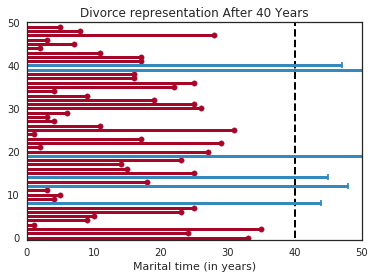
\includegraphics[height=2.1in,width=3.2in]{censorship.png}
\end{tabular}
\caption{Censoring Survival Data}
\label{Fig:Censoring}
\end{figure}\\
\section{Survival Analysis}
The survival function is used to represent the probability that the time to the event  is not earlier than a specified time $t$ \cite{klein2005survival} which is one of the primary goals in survival analysis. Conventionally, survival function is represented by $S(t)$,and it is given as follows:
\begin{equation}
S(t) = P(T \geq t)
\end{equation} 
The survival function of marriage monotonically decreases with $t$, and the initial probability value is 1 when $t$ = 0, which represents the fact that, in the beginning of the observation, 100\% of the observed couples survive; in other words, no events of divorce have occurred yet. On the contrary, the cumulative death distribution function $F(t)$, which represents the probability that the divorce occurs earlier than $t$, is defined as $F(t) = 1 - S(t)$. The probability density function $f(t)$ is expressed as $f(t)= F'(t)$ where $f(t)$ is continuous at time $t$.
\subsection{Estimating the survival time of marriage}
To estimate the survival time of marriages, we use the Kaplan-Meier estimator also known as the product limit estimator an non-parametric regression model, defined:
\begin{equation}
\hat{S}(t) = \prod_{i:t_{i} \leq t} \frac{n_i - d_i}{n_i}
\end{equation}
with $t_{i}$ a time when at least one event happened, $d_i$ the number of divorces that happened at time $t_{i}$ and  $n_{i}$ the couples who have not yet had an event of divorce or been censored at time $t_{i}$.
We see in Figure 3 that after 40 years of marriage only 30\% of couples make it together while the curve starts to stabilize when reaching 60 years with a probability of only 15\% of couples who would make it so far, the number decreases monotonically over time.\\
In Python, we use the KaplanMeierFitter method to fit the model to the data, after calling the fit method we plot the Kaplan-Meier's \textbf{`survival\_function\_'} as showing in the code below:
\lstinputlisting[language=Python, firstline=192, lastline=195]{Project.py}
\begin{figure}[!htb]
\centering
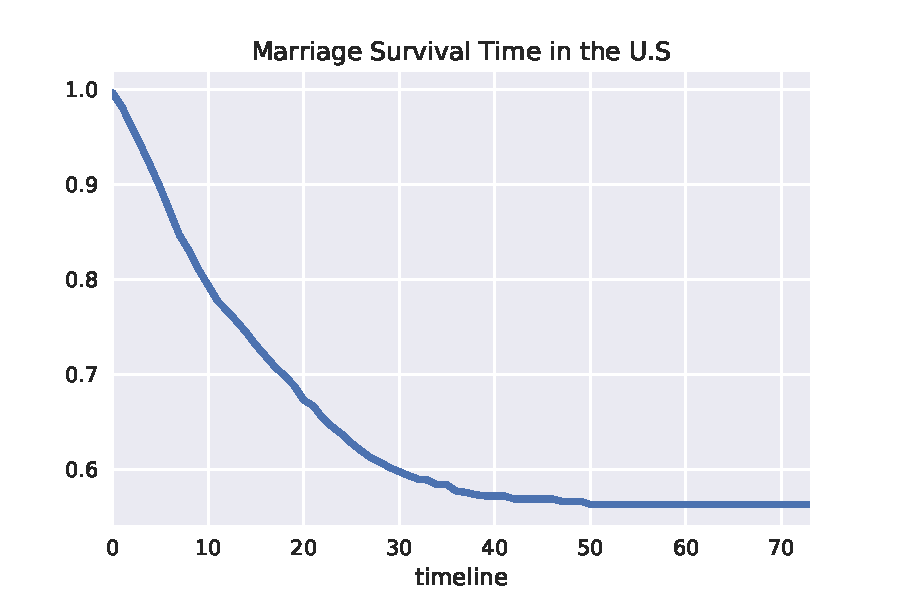
\includegraphics[scale=.64]{Survival.pdf}
\caption{Estimated Survival Time of Marriage}
\label{Fig:Survival_Time}
\end{figure}
\subsection{Ethnicity and Social Diversity}
In order to understand the marriage and its complicated social factors, we segregate the covariates of our dataset and plot the survival based on couple race to measure the effect of ethnicity on marriage longevity. This time we used KaplanMeierFitter object directly to plot the estimate which allow us to see the confidence intervals, we notice that this intervals becomes wider as the time increases which makes the prediction of marriage survival less accurate and the margin of error bigger. Results in Figure 4 shows that same-race couples are likely to survive together longer than mixed-race couple due to cultural discord or disagreement in beliefs \cite{falicov1998cultural}.
Implementation in Python looks as follows:
\lstinputlisting[language=Python, firstline=198, lastline=198]{Project.py}
\begin{figure}[!htb]
\centering
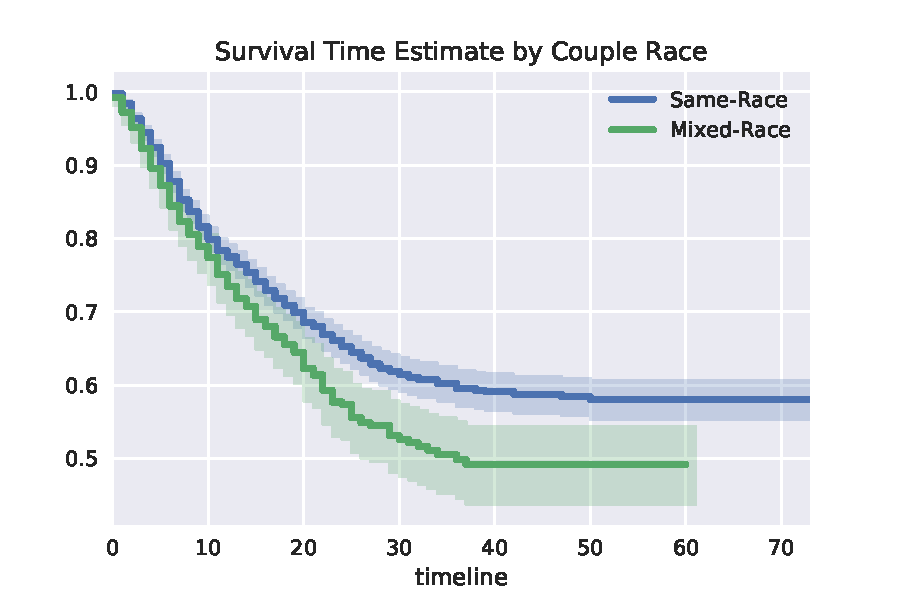
\includegraphics[scale=.64]{Couple_Race.pdf}
\caption{Estimated Survival Time of couple race}
\label{Fig:Survival_Time_Couple_Race}
\end{figure}
Similarly, The results in Figure 5 show that the scarcity of employed black men increases the chance of divorce in black communities. In turn, black family disruption substantially increases the rates of black murder and robbery, especially by juveniles. These effects are independent of income, region, race and age composition, density, city size, and welfare benefits and are similar to the effects of white family disruption on white violence. The paper concludes that there is nothing inherent in black culture that is conducive to crime. Rather, persistently high rates on black crime appear to stem from the structural linkages among unemployment, economic deprivation, and family disruption in urban black communities\cite{sampson1987urban}.
\begin{figure}[!htb]
\centering
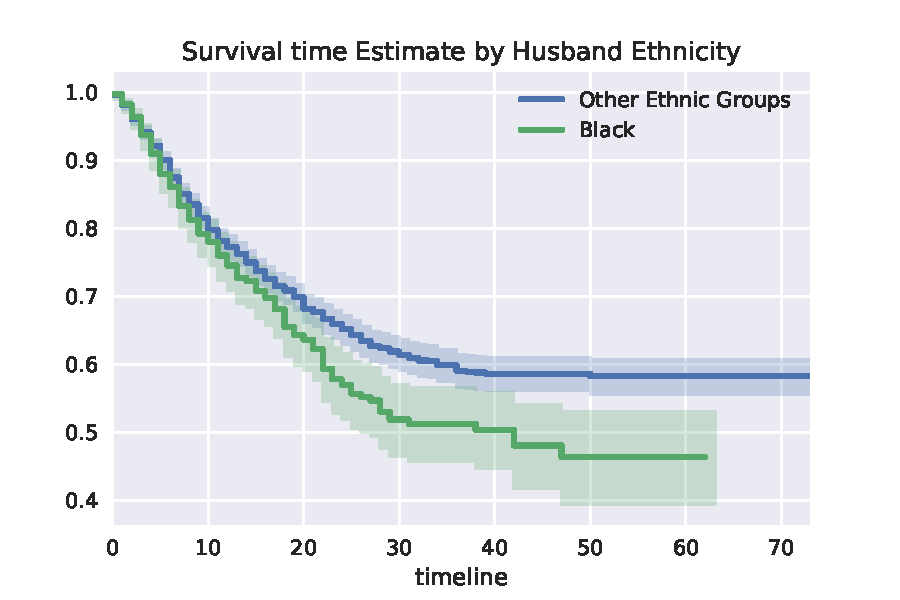
\includegraphics[scale=.64]{Ethnicity.pdf}
\caption{Estimated Survival Time by Ethnicity}
\label{Fig:Survival_Time_Ethnicity}
\end{figure}

\subsection{The Role of Eduction}
Separate estimates by educational attainment reveal a new socioeconomic pattern of marriage survival. Whereas in the  past,couples with more education were less likely to marry, recent college graduates are now forecast to marry at higher levels despite their later entry into first marriage.
\begin{figure}[!htb]
\centering
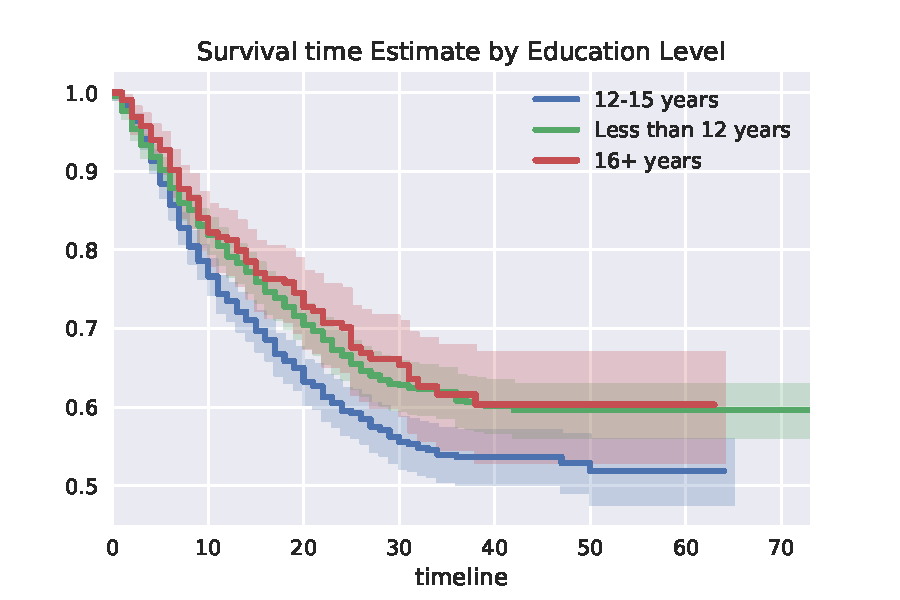
\includegraphics[scale=.64]{Education_level.pdf}
\caption{Estimated Survival Time by Education level}
\label{Fig:Survival_Time}
\end{figure}
Figure 6 explains the fact that well educated people has a slightly longer survival time than those who barely finished their primary education, the educational crossover which occurs for both black and white couples suggests that marriage is increasingly becoming a province of the most educated, a trend that may become a new source of inequality for future generations for couples who have 12 -15 years of education, according to the authors in \cite{goldstein2001marriage}.Segregation of education level categories is implemented in Python as below:
\lstinputlisting[language=Python, firstline=222, lastline=227]{Project.py}

\subsection{Geographical Location}
Economic data have been collected in 4 states in the U.S. as follows : Maryland, New Hampshire considered among the top richest states, while Mississippi and Alabama are in the bottom of the poorest states, the states were chosen based on their income ranking. We pulled average pay for each state, based on 2016 median household income from the Census Bureau's American Community Survey. Then we adjusted those figures based on each state’s 2017 regional price parity calculation. According to the calculation, we estimated marriage survival in each state based on their average pay using Kaplan-Meier estimator, the predictions were in favor of couples residing in the richest states of Maryland and New Hampshire followed by the ones in the poorest states of Mississippi and Alabama. To maximize our understanding of results, individual plots of each state have been displayed in order to compare (See Figure 7 and 8).
\begin{figure}[!htb]
\centering
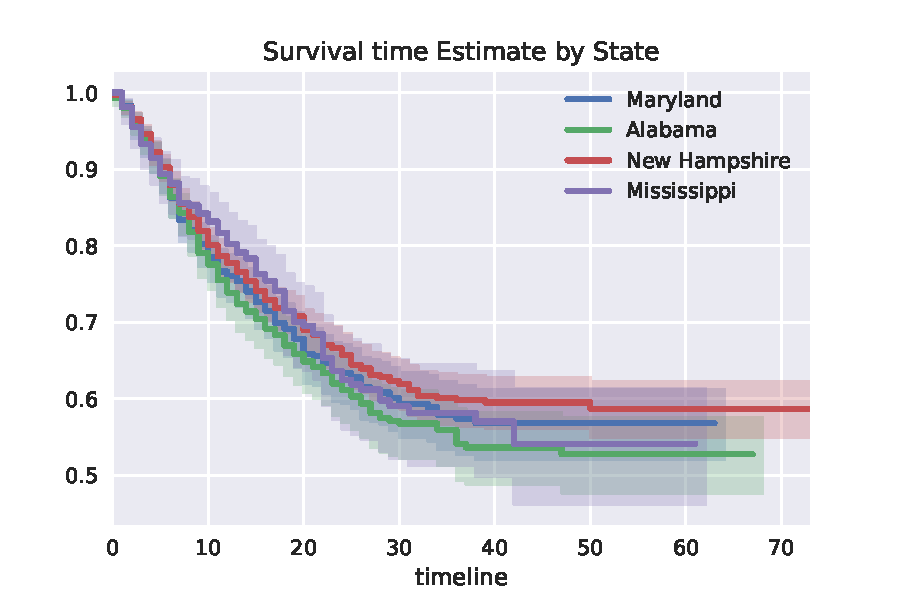
\includegraphics[scale=.64]{State.pdf}
\caption{Estimated Survival Time of 4 States}
\label{Fig:Survival_Time_State}
\end{figure}
\lstinputlisting[language=Python, firstline=253, lastline=260]{Project.py} 
\begin{figure}[!htb]
\centering
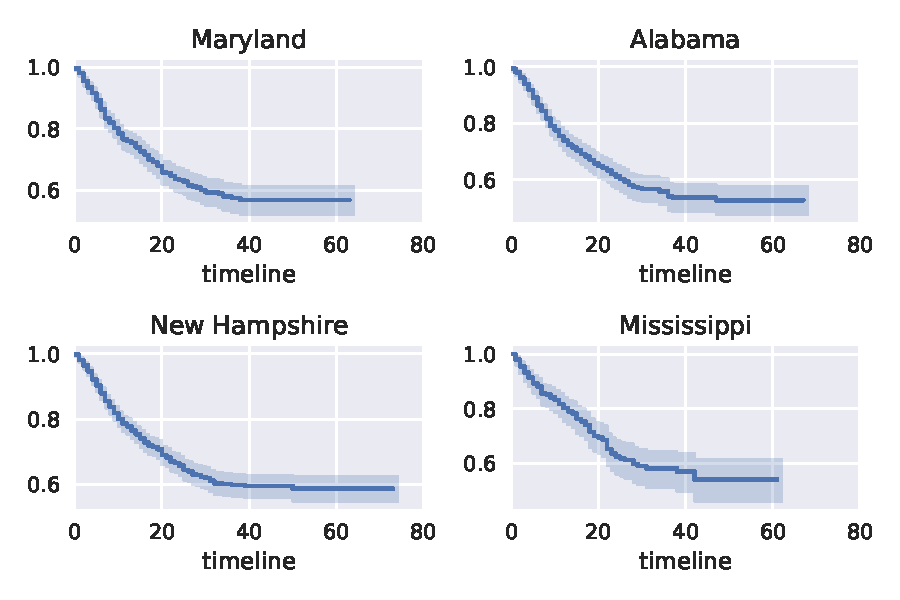
\includegraphics[scale=.64]{Marriage_States.pdf}
\caption{Estimated Survival Time by State}
\label{Fig:Survival_Time_State}
\end{figure}

\subsection{Income and Children}
An important role of income in marriage survival is found during the analysis. Due to the significant differences between economic classes, high earnings capacity increases the probability of marriage survival and decreases the probability of divorce for old couples. On the other hand, high earnings capacity decreases the survival time for young couples, Burgess et al described the important impact of income on the household welfare and composition\cite{burgess2003role}. We fit Kaplan-Meier estimator based on household income to produce results shown in Figure 9:
\lstinputlisting[language=Python, firstline=275, lastline=284]{Project.py} 
\begin{figure}[!htb]
\centering
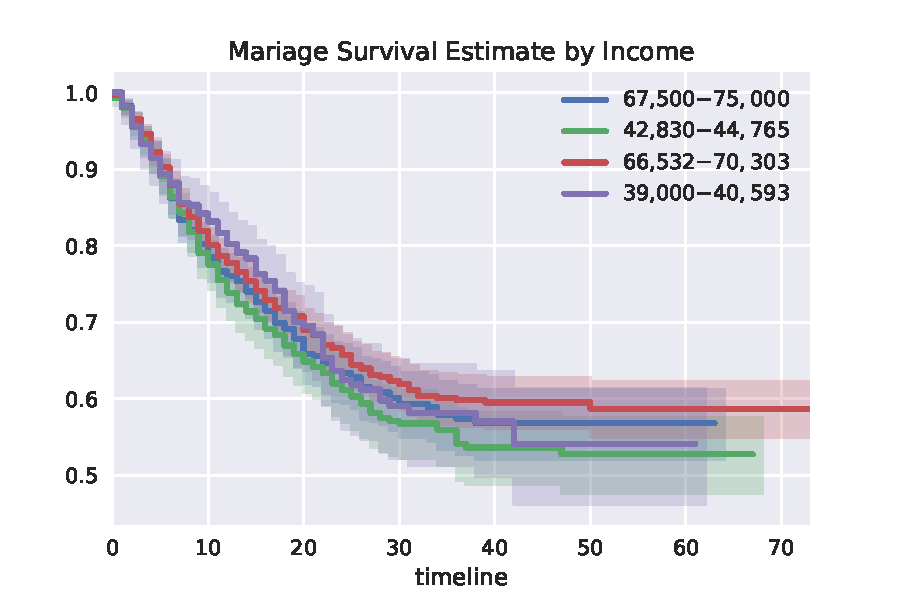
\includegraphics[scale=.64]{Household_Income.pdf}
\caption{Estimated Survival Time by Income}
\label{Fig:Survival_Household_Income}
\end{figure}
We found that, among young couples, teenage parenthood appears to increase the risk of divorce or separation, similarly to teenage marriage which significantly raises the probability of disruption. When the analysis was performed separately by race, this pattern held among white couples; however, for black couples a first birth before the age of 20 was found to increase instability more than a first marriage before that age. The finding that  age at first birth  but not age at first marriage is significantly related to the probability of marital dissolution appears robust in the total sample. As a conclusion, couples having children are more likely to be prone to divorce than the ones who doesn't have children yet. To generate the corresponding results in Figure 10, we include Python code below for more details:
\lstinputlisting[language=Python, firstline=288, lastline=293]{Project.py} 
\begin{figure}[!htb]
\centering
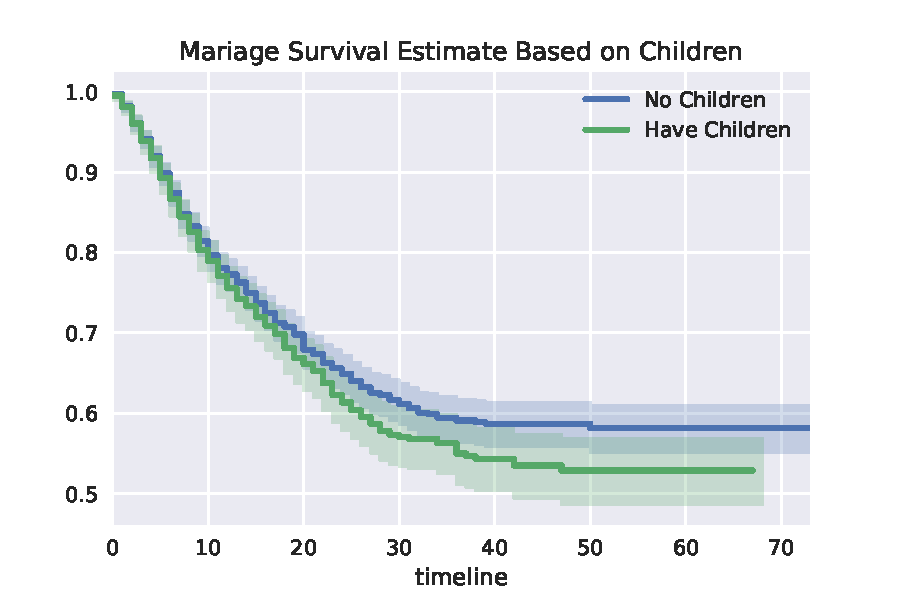
\includegraphics[scale=.64]{Children.pdf}
\caption{Estimated Survival Time based on Children}
\label{Fig:Survival_Household_Children}
\end{figure}
 \section{Hazard function}
The hazard function $h(t)$ is another aspect of survival analysis, which is also called the conditional failure rate \cite{dunn2009basic}. The hazard function indicates the rate of divorce at time $t$ given that no event occurred before time $t$. The hazard function is defined as:
\begin{equation}
h(t) = \lim_{\Delta{t} \to 0} \frac{P(t \leq T < t+\Delta{t} | T \geq t)}{\Delta{t}} 
\end{equation}
Statistically to represent hazard function of  our population in Python, we cannot transform the Kaplan Meier estimate or survival function into hazard function. However, a proper estimator of the cumulative hazard function called Nelson Aalen estimator is also a non-parametric estimator of the cumulative hazard rate function in case of censored data is used to quantify and plot the hazard given by:
\begin{equation}
\hat{H}(t) = \sum_{t_i \leq t} \frac{d_i}{n_i} 
\end{equation}
with $ d_{i}$ the number of divorce events at $ t_{i}$  and $n_{i}$  is the total number of couples at risk at $t_{i}$ in our study. Using lifelines package in Python, this estimator is available as the \textbf{NelsonAalenFitter} which used to fit the dataset and print the \textbf{'cumulative\_hazard\_'} summary that shows that more than 51.4\% of the population will experience divorce after 30 years of marriage :
\lstinputlisting[language=Python, firstline=298, lastline=302]{Project.py}
The cumulative hazard curve is less sensible to changes than the survival curve, however it is the building block of more sophisticated techniques in survival analysis such as Cox Proportional Hazard which we will explain in the next section. Since we are estimating cumulative hazard curve, the sum of estimates is always more stable than the point-wise estimates of a single couple. Thus we know the rate of change of this curve is an estimate of the hazard function.\\ Looking at figure Figure 11, it looks like the hazard starts off high and gets smaller and smaller as the hazard rate decreases.
\begin{figure}[!htb]
\centering
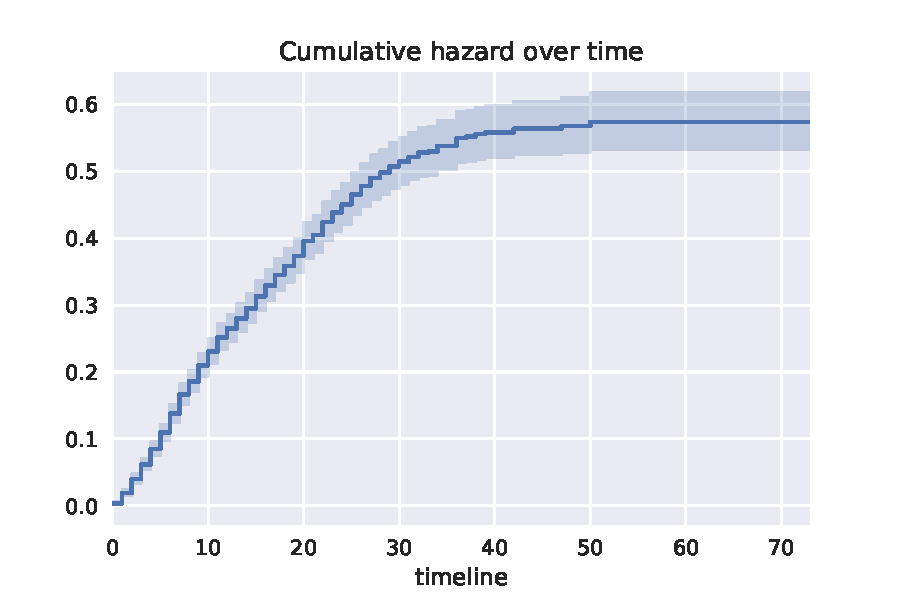
\includegraphics[scale=.64]{Cumulative_Hazard_function.pdf}
\caption{Estimated Cumulative Hazard}
\label{Fig:Estimated Cumulative Hazard}
\end{figure}
To see which covariate is causing more hazard than others, we broke the couples down between same-race and mixed-race couples, and plot the curves. The analysis shows that after 30 years of marriage, 64.5 \% of mixed-race couples will get divorced while 49.8 \% of same-race couples will be divorced by that time (See Figure 12).  As a complimentary function to the survival function plot of husband race, the cumulative hazard function shows that 67.3\% of couples headed by black males are prone to get divorced comparing to 50\% of other ethnic groups after 30 years of marriage. All results could be retrieved from the cumulative\_hazard\_ as mentioned earlier using Lifelines in Python (See Figure 13). 
Based on the results of Economic data that have been collected in 4 states in the U.S and analyzed using survival analysis earlier in this study, we plot the cumulative hazard function again, this time using the state segregation in order to obtain more information about the best place for a household to choose to live in and to predict the best welfare and social net condition to help guide couples in establishing their families with the minimum economic and social challenges.\\  
\begin{figure}[!htb]
\centering
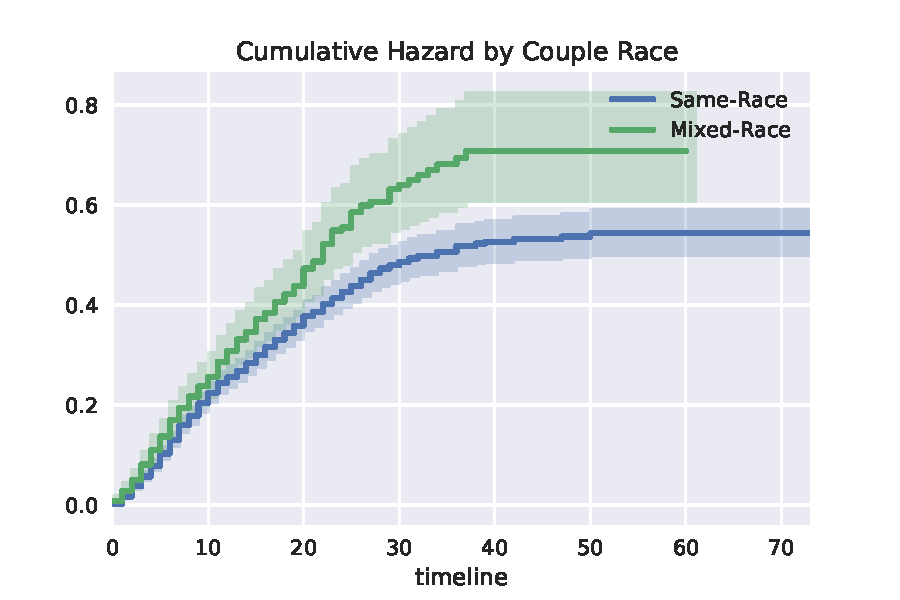
\includegraphics[scale=.64]{Cumulative_Hazard_CoupleRace.pdf}
\caption{Estimated Cumulative Hazard by Couple Race}
\label{Fig:Estimated Cumulative Hazard Couple Race}
\end{figure}
\begin{figure}[!htb]
\centering
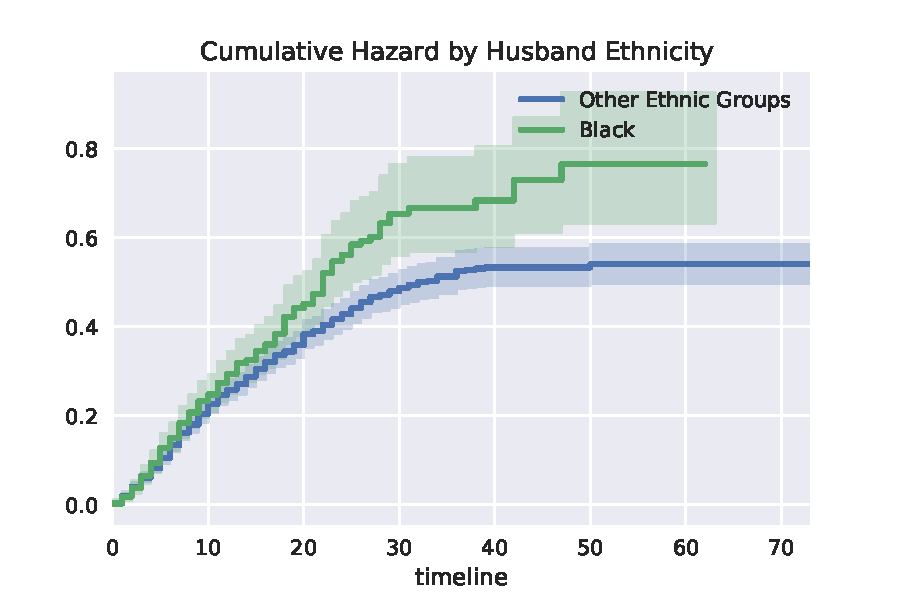
\includegraphics[scale=.64]{Cumulative_Hazard_HusbandRace.pdf}
\caption{Estimated Cumulative Hazard}
\label{Fig:Estimated Cumulative Hazard}
\end{figure}
\\In Figure 14 we found that the results of the cumulative hazard prediction are aligned with the prior information that we have on these states, the curves show that the two richest states: New Hampshire and Maryland have the lower hazard rates. On the contrary, the two poorest states: Mississipi and Alabama obtained a higher classification according to their hazard prediction based on the median household income and their annual average pay. In a comparative snapshot, at time $t_i$=$40$ years, 38\% of couples who are living in New Hampshire will experience divorce, while 50\%  of couples living in Maryland will experience divorce at same time. The number is slightly higher in the state of Mississippi where 53.5\% of couples will be divorced and finally the higher percentage of divorce is in Alabama with 57.3\%. As a conclusion of this analysis, New Hampshire is the best place to start a family based on Nelson-Aalen estimator.
\begin{figure}[!htb]
\centering
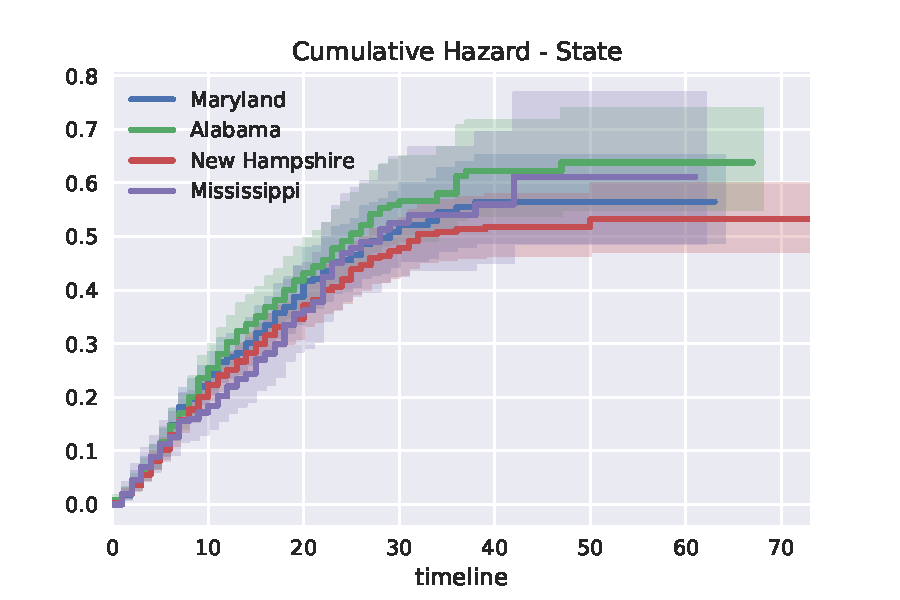
\includegraphics[scale=.64]{Cumulative_Hazard_State.pdf}
\caption{Estimated Cumulative Hazard}
\label{Fig:Estimated Cumulative Hazard}
\end{figure}
\section{Survival Regression}
Survival analysis focuses on characterizing both the distributions of the event times and the statistical properties of the parameter estimation by estimating the survival curves, they are generally developed for the low-dimensional data.The traditional statistical methods in survival analysis can be subdivided into three categories: (i) nonparametric models \cite{kaplan1958nonparametric}, (ii) semi-parametric models  and (iii) parametric models \cite{cutler1958maximum}. 
\subsection{Semi-Parametric Models}
In this study, we are interested in using semi-parametric models of survival analysis for prediction. The most commonly used regression analysis approach for survival data is the Cox Proportional Hazard model as semi-parametric model, it differs significantly from other methods since it is built on the proportional hazards assumption and employs partial likelihood for parameter estimation. The distribution of the outcome remains unknown even if it is based on a parametric regression model. In addition, several useful variants of the basic Cox model, such as penalized Cox models, Cox-Boost algorithm and Time-Dependent Cox model (TD-Cox), are considered an extension to this popular model.  As a hybrid of the parametric and non-parametric approaches, semi-parametric models can obtain a more consistent estimator under a broader range of conditions compared to the parametric models, and a more precise estimator than the non-parametric methods \cite{powell1994estimation}. Unlike parametric methods, the knowledge of the underlying distribution of time to event of interest is not required, but the attributes are assumed to have an exponential influence on the outcome. 
\subparagraph{•}
\textbf{Cox Proportional Hazard Model}.The purpose of the model is to evaluate simultaneously the effect of several factors on survival. In other words, it allows us to examine how specified factors influence the rate of a particular event happening (e.g., infection, death) at a particular point in time. This rate is commonly referred as the hazard rate. Predictor variables (or factors) are usually termed covariates in the survival-analysis literature.
The Cox model is expressed by the hazard function denoted by h(t). Briefly, the hazard function can be interpreted as the risk of dying at time $t$. It can be estimated as follow:
\begin{equation}
h(t, X) = h_0(t)\exp(\beta_1 X_1 + \beta_2 X_2 + ...+\beta_p X_p ), 
\end{equation}
where $t$ represents the survival time, $h(t)$ is the hazard function determined by a set of $p$ covariates $(X_1,X_2,...,X_p)$, the coefficients $(\beta_1,\beta_2,...,\beta_p)$ measure the impact (i.e., the effect size) of covariates. The term $h_0$ is called the baseline hazard. It corresponds to the value of the hazard if all the $x_i$ are equal to zero.\\
\\The Cox model can be written as a multiple linear regression of the logarithm of the hazard on the variables $x_i$, with the baseline hazard being an ‘intercept’ term that varies with time. The term $\exp(b_i)$ are called hazard ratios ($HR$). A value of $b_i$ greater than zero, or equivalently a hazard ratio greater than one, indicates that as the value of the $i^th$ covariate increases, the event hazard increases and thus the length of survival decreases.  For any two instances $X_1$ and $X_2$, the hazard ratio is given by:
\begin{equation}
\dfrac{h(t,X_1)}{h(t,X_2)} = \dfrac{h_0(t)\exp(\beta X_1)}{h_0(t)\exp(\beta X_2)} = \exp[(X_1 - X_2)\beta].
\end{equation}
Which means that the hazard ratio is independent of the baseline hazard function. Cox model is a proportional hazards model since the hazard ratio is a constant and all the subjects share the same baseline hazard function.\\
In Lifelines, Cox proportional Hazard model is implemented using \textbf{CoxPHFitter} that has a `\textit{print\_summary}' function similarly to Kaplan-Meier and Neslson-Aalen models which prints statistical coefficients in a tabular view as below:
\lstinputlisting[language=Python, firstline=512, lastline=517]{Project.py}
\begin{figure}[!htb]
\centering
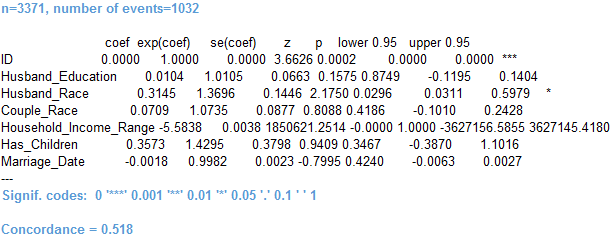
\includegraphics[height=2.0in,width=3.5in]{CPH_Coefficients_Table.PNG}
\caption{CPH Coefficients Summary}
\label{Fig:CPH_Coefficients_Table}
\end{figure} 
Fitting the model took 13 iterations to complete the convergence of covariates in our dataset, the \textit{`show\_progress'} parameters allows us to see the progress. After fitting CPH model, we want to know how accurate is our model was to the data. A common way to evaluate a model is to consider the relative risk of an event for different instance instead of the absolute survival times for each instance, this popular metric is designated by Concordance-index.The C-index calculated at the bottom of the summary table is equal to $0.548$. It means that CPH model slightly outperforms average performance for our data. An alternative way to view the coefficients and their ranges is to visualize it using the plot method in CPH, that will give us a better idea which covariate affects the dataset the most and in which range it falls.\\
Results in Figure 16 show that it is  obvious to conclude that the covariate `Has\_children' is the most important feature in our dataset, the existence of children in the family affects drastically the survival time of marriage, followed by husband race, couple race and income average per year. Surprisingly, poverty percentage of each state has a minor influence on household welfare.
\begin{figure}[!htb]
\centering
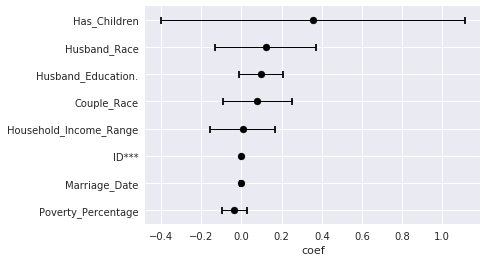
\includegraphics[height=2.0in,width=3.5in]{CPH_Coefficients_Plot.PNG}
\caption{CPH Coefficients Plot}
\label{Fig:CPH_Coefficients_Plot}
\end{figure}
The partial likelihood is the product of the probability at each event time $T_i$ that the event has occurred to individual $i$, given the set of individuals still at risk at time $T_i$. The Cox partial likelihood is parameterized by $\beta$ and defined as:
\begin{equation}
L(\beta) = \prod_{j=1}^{N}\left[\frac{\exp^{(X_j\beta)}}{\sum_{i \in R_j}\exp^{(X_i\beta)}}\right]^{\delta_j}
\end{equation}
here $j=1,2,...,N$; if $\delta_j = 1$, the $j^{th}$ term in the product is the conditional probability; otherwise, when $\delta_j$ = 0, the corresponding term is 1, which means that the term will not have any effect on the final product. The coefficient vector $\hat{\beta}$ is estimated by maximizing this partial likelihood, or equivalently, minimizing the
negative log-partial likelihood for improving efficiency.
\begin{equation}
\label{eq:equation8}
LL(\beta) = -\sum_{j: E_j=1} \delta_j\bigg( \hat{h}_{\theta }(X_j) - \log \sum_{i \in \mathbb{\Re}_j}\exp^{\hat{h}_{\theta }(X_i)}\bigg). 
\end{equation}
In python, an easy way to check the proportional hazards assumption of a variable is to compare the survival curves segmented by the values of the variable. If the survival curves are the same shape and differ only by a constant factor, then the assumption holds. KaplanMeierFitter object has a `plot\_loglogs' function for this purpose which uses the logs curve or the loglogs given in ~\ref{eq:equation8} to plot proportional hazards. If the curves are parallel and do not cross each other, then it is likely the variable satisfies the assumption. If the curves do cross, then we have stratify the variable.\\ 
\begin{figure}[!htb]
\centering
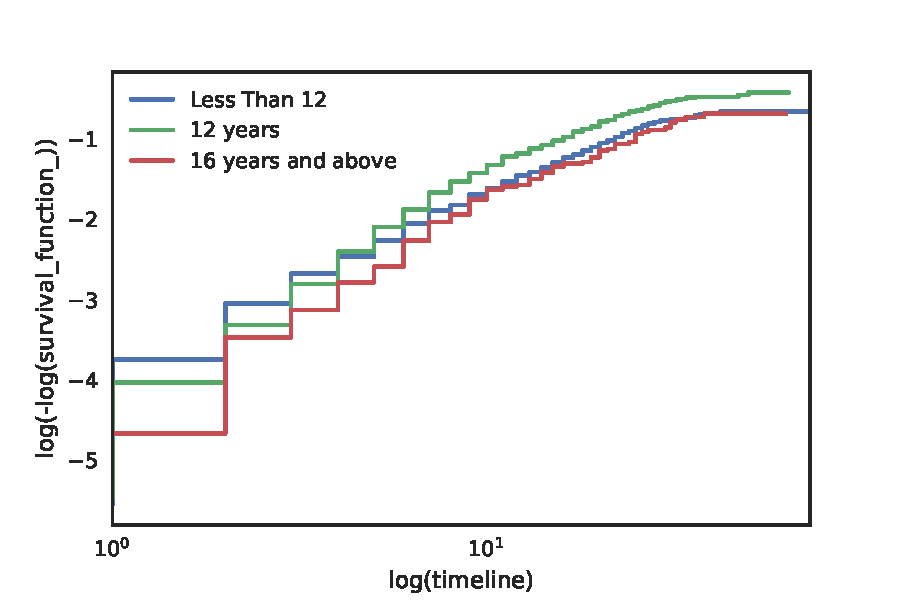
\includegraphics[scale=.64]{CPH_Pproportional_Hazards_Assumption.pdf}
\caption{Proportional Hazards Assumption}
\label{Fig:Pproportional_Hazards_Assumption}
\end{figure}
The analysis of Figure 17 led us to many conclusions. First, when we tried to plot the proportional hazard assumption of educational level, the curves cross each other, more specifically between the "12 years" value (green curve) and "Less than 12" value which means that the variable doesn't satisfy the assumption. Therefore we tried to stratify this variable based on the most weighted variable according to Figure 16. Hence, we used the variable "Has\_Children" in order to acquire more information about impact of education on our population and that enhances the C-index by increasing to 0.623. Code provided below:
\lstinputlisting[language=Python, firstline=596, lastline=598]{Project.py}
Finally, we calculate the correlation between all variables and then we visualize it using Seaborn package in Python to display the relationship between all covariates and its impact on the marriage dataset, code provided below:
\lstinputlisting[language=Python, firstline=523, lastline=524]{Project.py}
\begin{figure}[!htb]
\centering
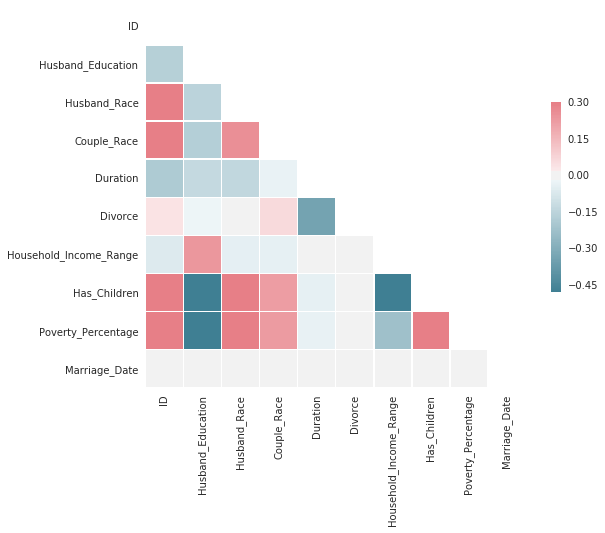
\includegraphics[scale=.43]{CPH_Triangle_Correlation.png}
\caption{Correlation Triangle}
\label{Fig:CPH_Triangle_Correlation}
\end{figure} 
\textbf{Aalen Additive Hazard Model}.
Based on our findings, the proportional hazard assumption was not satisfied, in this case Aalen's additive model is an appropriate alternative for the Cox model. A conceptually similar model to CPH, this model is easier to work with at the cost at some other problems, Intensity for $N(t), t \in  [0,\tau ], \tau < \infty$, of a subject with a p-dimensional covariate, $X(t) = (X_1(t), ..., X_p(t))^T$, and at risk indicator, $Y (t)$, is on the form:
\begin{equation}
\lambda(t) = Y(t)X^T(t)\beta(t) = Y(t)\sum_{j=1}^PX_j(t)\beta_j(t) 
\end{equation}
then calculating the cumulative regression coefficients of  Aalen-Additive hazard model can be easy:
\begin{equation}
B(t) = \int_0^t \beta(s)ds
\end{equation} 
Translating the equation above in Python, the estimator to fit unknown coefficients in Aalen’s additive model is located under AalenAdditiveFitter. In our study, we will use the marriage dataset and include the categorical variables:\texttt{State, Couple Race,Household Income}, the husband's education level  (i.e.:\texttt{ less than 12 years, 12 years,more than 16 years}) and the year the marriage started in, \texttt{Marriage\_Date}. 
Aalen’s additive model typically does not estimate the individual $b_i(t)$ but instead estimates the additive hazard similarly to the estimate of the hazard rate using NelsonAalenFitter above. Using patsy library in Python to create a covariance matrix from original dataframe before fitting the model:
\lstinputlisting[language=Python, firstline=395, lastline=404]{Project.py}
During the estimation, a linear regression is computed at each step. Often the regression can be unstable due to high co-linearity and the relative small size of our dataset, we can add a “penalizer” parameter to control the stability which recommended to start with a small Penalizer in case the estimates still appear to be too unstable, and then we try to increase it gradually.
\begin{figure}[!htb]
\setlength{\tabcolsep}{.000001em}
\centering
\begin{tabular}{cc}
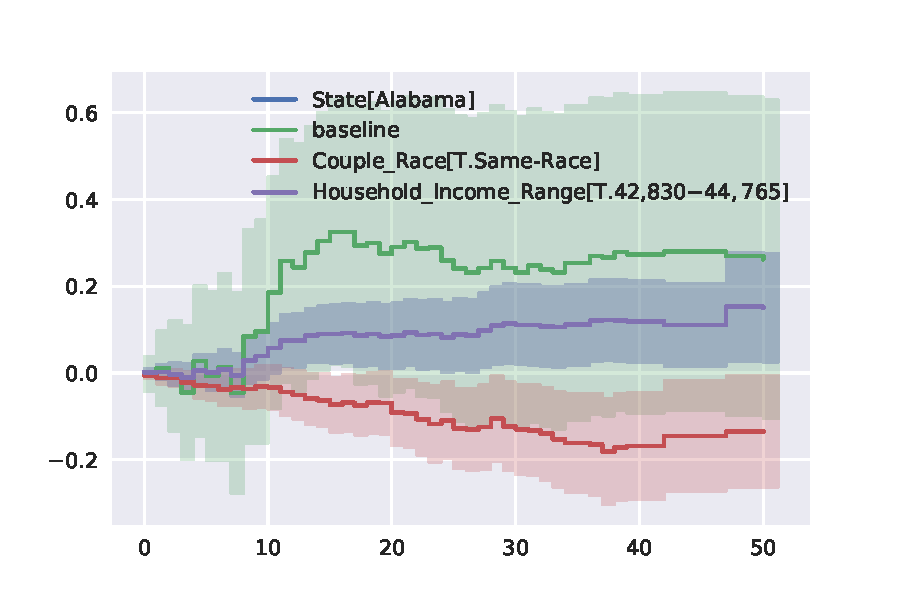
\includegraphics[width=1.85in,height=1.5in]{Survival_Regression_for_Alabamae.pdf} &
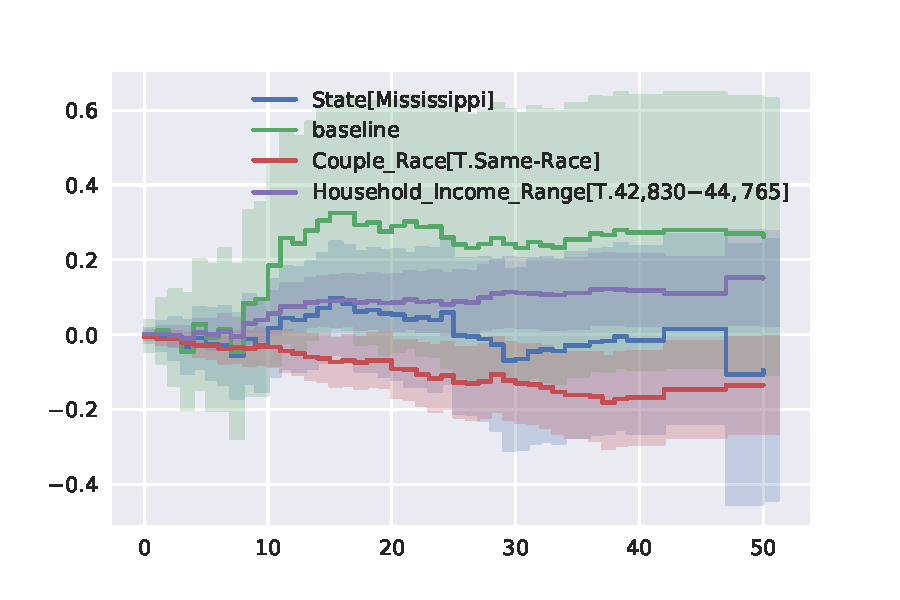
\includegraphics[width=1.85in,height=1.5in]{Survival_Regression_for_Mississippi.pdf}\\
Alabama &   Mississippi\\
\\
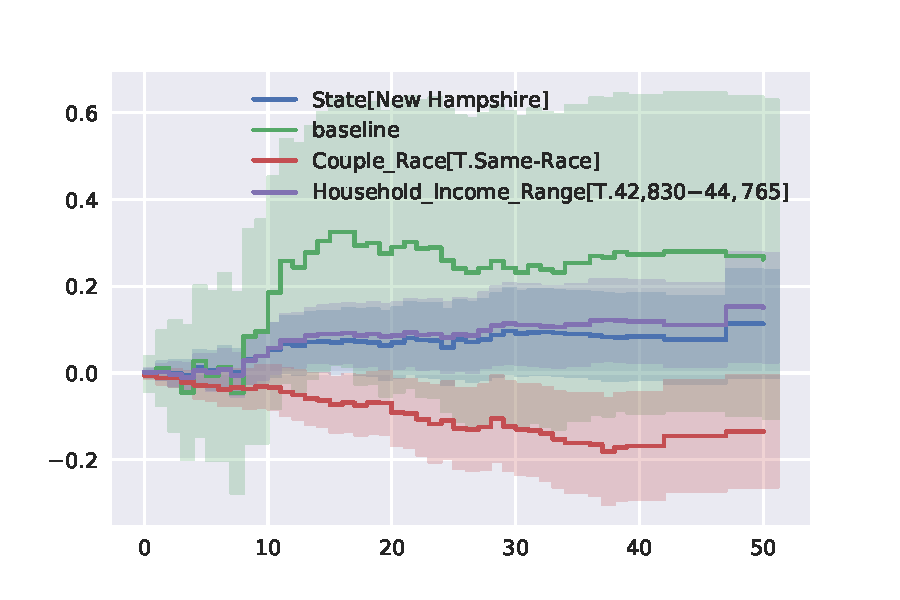
\includegraphics[width=1.85in,height=1.5in]{Survival_Regression_for_New_Hampshire.pdf}&
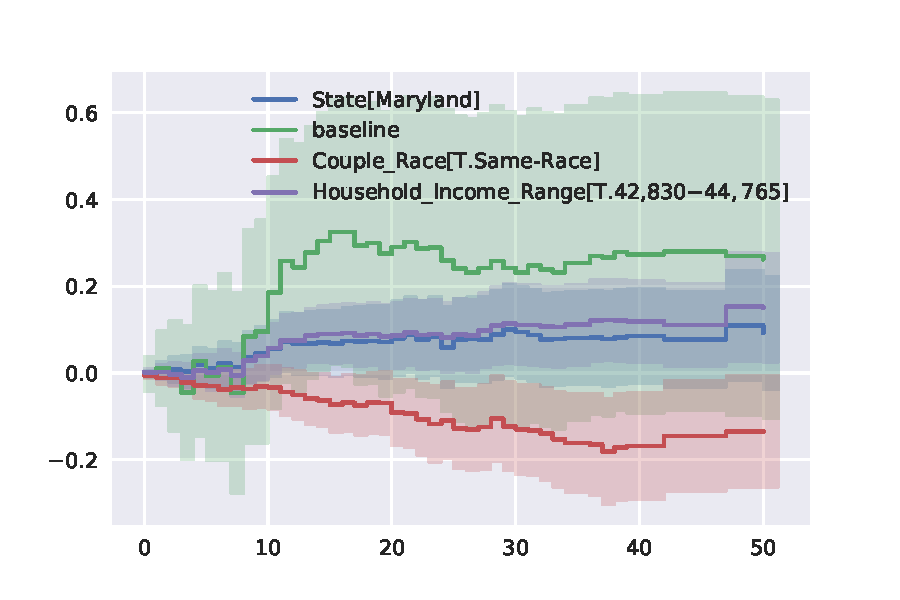
\includegraphics[width=1.85in,height=1.5in]{Survival_Regression_for_Maryland.pdf}\\
New Hampshire &  Maryland\\
\end{tabular}
\caption{Survival regression in each state }
\label{Fig:predicted_hazard}
\end{figure}\\
In New Hampshire and Maryland, the estimated hazard related to couple race and income are closer to the baseline hazard than the one estimated for the states of Alabama and Mississippi, which means that the model is capable of predicting a better life conditions based on income, race diversity and geographical location, we take Maryland state as an instance. The estimated hazard for Alabama is much higher than any other place which makes it the least preferable place in our study to establish a family based on the prediction.\\
Regression is most interesting if we use it on data we have not yet seen,in machine learning we call it the testing dataset.  Therefore, we can use what we have learned so far from our covariates to predict individual hazard rates or  survival time of a specific couple and compare it to other couples in different states under the same circumstances to gain more insight about individual behavior of marriage. The \texttt{Mariage\_Date} of couples is available up until 2016,so we use this data to predict the possible duration of couples who get married in 2016  (though already partly seen)  in the 4 different states which we are studying. First we select 4 random couples married in 2017 each of which from a different state,then we subset the dataframe \texttt{data} to a smaller dataframe of 4 couples only and compare our prediction outputs as shown in Figure 19.
\begin{figure}[!htb]
\setlength{\tabcolsep}{.000001em}
\centering
\begin{tabular}{cc}
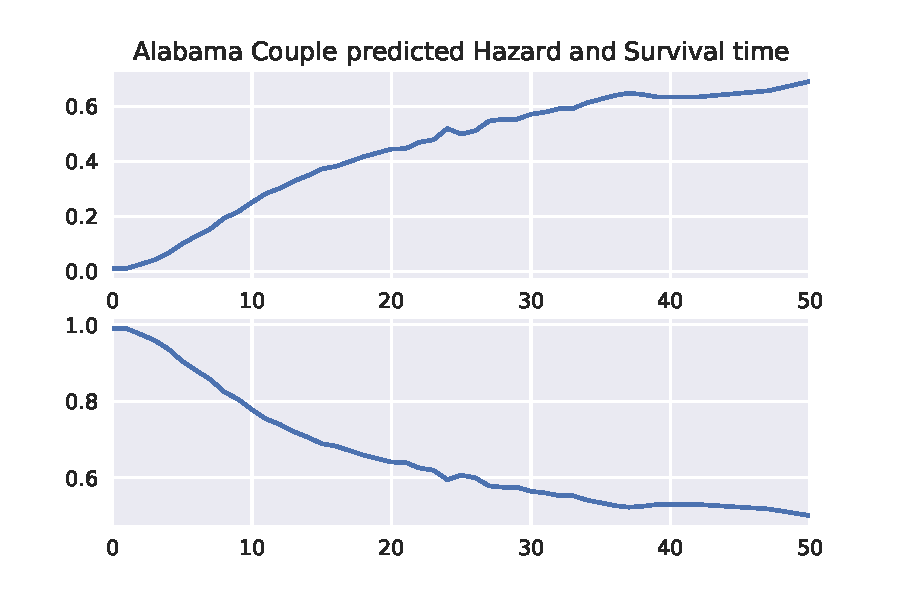
\includegraphics[width=1.85in,height=1.5in]{AlabamaCouple.pdf} &
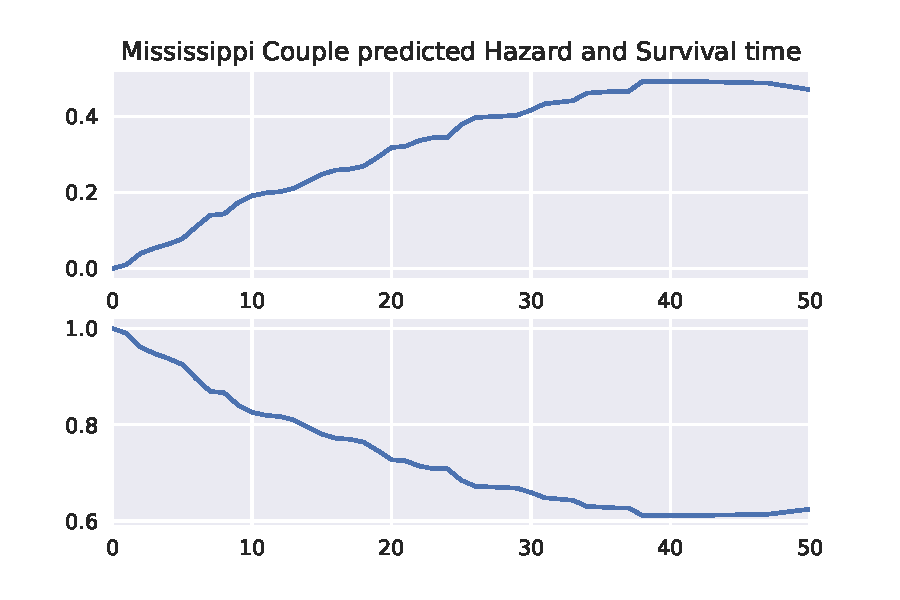
\includegraphics[width=1.85in,height=1.5in]{MarylandCouple.pdf}\\
Alabama &   Mississippi\\
\\
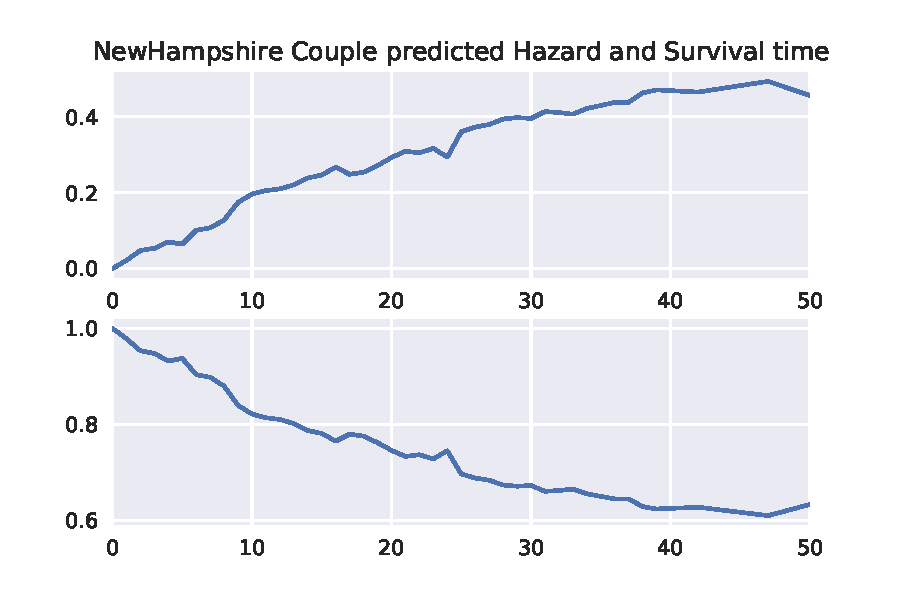
\includegraphics[width=1.85in,height=1.5in]{NewHampshireCouple.pdf}&
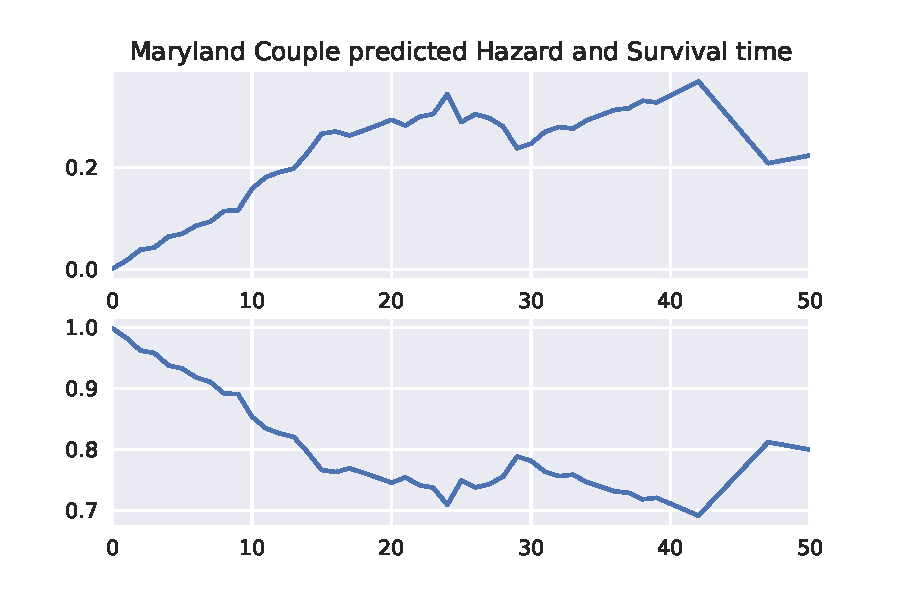
\includegraphics[width=1.85in,height=1.5in]{MississippiCouple.pdf}\\
New Hampshire &  Maryland\\
\end{tabular}
\caption{Individual predicted hazard and survival time }
\label{Fig:predicted_hazard}
\end{figure}\\
Predicted hazards for couples living in Alabama and Mississippi are obviously the highest among all others hence the survival time is shorter. We can also notice that New Hampshire has a stable prediction of hazard and survival time while the situation in Maryland is depending heavily on the conditions of other social and economic factors, however the latter showed a longer survival time than New Hampshire.
\section{Conclusion}
Present study attempt to understand the associated factors affecting the marriage dissolution in the U.S.in general and also separately by 4 states : New Hampshire, Maryland, Alabama and Mississippi.A part of the dataset has been used in the analysis is one of the largest demographic data source of the United States Census Bureau survey on poverty, covering all the districts of country, along with provincial data from Princeton University database. The hazard regression analyses suggest that  region, place of residence,children ever born, both the partner’s education had significant effects on the chances of marriage dissolution. Educated husbands have higher chances of marriage dissolution than the illiterate ones. Regional analysis depicts variations among the states. The regional analysis is important to understand the marriage dissolution pattern in various states in the U.S. which showed huge regional diversity in socio cultural status,  marriage pattern, ethnicity, etc. Regional differences in marriage patterns have been observed during 1970-2016 and concluded that states of Alabama and Mississippi had the highest marriage dissolution rates. The rest of the covariates varies by state, but the number of divorce cases in the U.S. is rising ,hence it becomes important to focus on the issue of marriage dissolution which affect individuals well being and their family life. Many studies conducted on consequences of divorce reveal that divorced persons as compared to married persons experience low level of psychological well being, poor self esteem, low happiness, psychological distress, (Aseltine \& Kessler \cite{aseltine1993marital}; Davies et al.\cite{scherzinger1997huntingtin}; Demo \& Acock \cite{david1996family}; Lorenz et al. \cite{lorenz1997cognitive}; Marks \cite{marks1996european}; Johnson and Wu \cite{johnson2002empirical}). Divorced persons experience poor health condition than the married ones, further it leads to greater mortality (Aldous \& Ganey \cite{aldous1999family}; Hemstrom \cite{hemstrom1996marriage}; Smith \cite{smith2008social} ).
\section*{Acknowledgments}
I would like to express my gratitude to my supervisor, Dr. A. Ben Hamza, for his continuous support, motivation and advice he has provided throughout the time of the project. 
\bibliographystyle{ieeetr}
\bibliography{Bib} %references

\end{document}